\chapter{Event reconstruction}\label{chap:Rec}
\minitoc
Raw detector information can not be used directly in the physics analysis. The reconstruction allows interpreting the electronic signals as parameters of physics objects. Event reconstruction is used to identify the particles, estimate their momenta and interaction vertices. In this chapter, the reconstruction and identification of the physics objects used in the \atlas experiment is described. 

Since this analysis presents the measurement of $W\to l\nu$ and $Z \to ll$ cross sections in both the electron and muon channels, the reconstruction of identification of electrons (Sec.~\ref{sec:ElecRec}) and muons (Sec.~\ref{sec:MuonRec}) are discussed in details. The missing transverse energy (\etmiss), that acts as an approximation for neutrino transverse momentum from $W$ decays, is described in Sec.~\ref{sec:EtMissRec}. It should be noted, that the standard \etmiss reconstruction used in the \atlas experiment was not applicable in the dataset used in the analysis and a different approach has been adapted.

\section{Tracks and vertices}

Tracks and vertices are reconstructed using the ID\cite{Track}. The reconstruction can be divided into 2 steps. 
On the first step, the inside-out algorithm is used based on the information from the pixel detector and SCT. Tracks are reconstructed from the set of 3 points called seed and then the new hit positions are added while moving closer to the interaction point using the iterative algorithm called Kalman filter\cite{Kalman}.  

Ambiguities in the track candidates are resolved in the final step and then the tracks are extended to the TRT position. In this step, algorithm searches for track segments reconstructed in TRT and then extends them into the pixel detector and SCT. Tracks reconstructed in TRT with no extension are referred to as TRT-standalone tracks. 

Interaction vertices are reconstructed using the iterative vertex finding algorithm. The vertex finding starts from the $z$-position at the beam axis of a random track. The fit based on\chiD minimisation is performed on that initial track and nearby tracks. Tracks, that are displaced by more than 7$\sigma$ from the vertex are used to form a separate vertex. The procedure is repeated until no new vertices are found.  The vertices are required to have contain at least two tracks. The  vertex with the highest sum of outgoing track momenta is defined as the \textit{primary vertex}.

\section{Electron reconstruction and identification}\label{sec:ElecRec}

The reconstructed electrons can be divided into two groups: central and forward. In the case of the central electrons ($| \eta |$ < 2.5) there is an ID tracking information available, which allows performing more precise reconstruction and identification. The forward   electrons (2.5 < $| \eta |$ < 4.9) are reconstructed using only the calorimeter information and a different electron reconstruction algorithm is used. In this section, the identification criteria of the central electrons and the reconstruction for both central and forward electrons, are discussed.

\subsection{Central electrons reconstruction}
Reconstruction of central electron starts from the EM cluster information.  The EM calorimeter clusters are formed from the cells with size $\Delta \eta \times \Delta \phi = 0.25 \times 0.25$ with total transverse energy in all calorimeter layers above 2.5 GeV using the sliding window algorithm\cite{ElecClust}. The position of the cluster is determined from the barycenter of the cluster.

In the second step, tracks with $P_{T}$ > 0.5 GeV are extrapolated to the middle layer of the EM calorimeter. A track is considered matched with a cluster if the distance track impact point and cluster position is  within $|\Delta\eta|$ < 0.05. In order to take into account effect of the bremsstrahlung losses, the azimuthal distance between track and cluster position is allowed to be $\Delta\phi$ < 0.1.

An electron is considered to be reconstructed if at least 1 track is matched to a given EM cluster. In case there are several tracks passing this requirement, the track with the smallest distance $\Delta R = \sqrt{\Delta\eta^2+\Delta\phi^2}$ is selected as the match. In case there is no track matched, the EM cluster is treated as a photon candidate.

After track-matching the cluster size is enlarged. The total reconstructed electron energy is determined from the corrected cluster energy, energy deposit in the material in front of EM calorimeter and energy deposits outside of the cluster and calorimeter. The relevant energy scale determination is described in Sec.~\ref{sec:elecScale}. The direction of the electron is determined from the corresponding track parameters. 


\subsection{Forward electrons reconstruction}

Since there is no tracking information in the forward region (2.5 < $|\eta|$ < 4.9), the electrons can be reconstructed using the information from EMEC and FCAL. The forward electrons reconstruction uses the topological clustering algorithm\cite{Lampl:1099735} with the variable cell size. In this algorithm, in cells with energy higher than the expected noise are merged together iteratively. The average noise in the cell is obtained in a dedicated (calibration) runs. The cluster building procedure starts from the cell having the significant large energy and then expands by neighborhood cells. If two clusters are sharing one neighboring cell, they are merged into a single cluster. 

The energy of the electron is defined as the sum of the cell energies, taking into account the energy losses in the passive material in front of the calorimeter. The direction of a forward electron is defined from the barycentre of associated cluster.

\subsection{Electron identification}

The application of additional selection criteria on reconstructed electrons allows excluding objects, that can be misidentified as electrons, such as jets and photons. 

The identification of the central electron is based on the sequential selection criteria based on calorimeter and tracking information. There are three sets of electron identification criteria, used for a physics analyses\cite{1404.2240}. They are ordered by the increasing background rejection at the cost of decreasing identification efficiency:
\begin{description}
\item[Loose] The loose identification criteria  uses the shower shape variables in the first and the second layer of EM calorimeter and the fraction of cluster energy, deposited in the hadronic calorimeter. There are also additional requirements on electron track and track-cluster matching;
\item [Medium] The medium selection is based on loose identification incorporating additional information from the 3-rd layer of EM calorimeter, transverse impact parameter of the electron candidate and TRT information. Additionally, a hit in the innermost layer of pixel detector is required to discriminate against the photon conversions. 
\item [Tight] In addition to medium criteria, this selection puts stricter requirements on electron track quality, on the ratio of EM cluster energy to electron track momentum, and on the reconstructed photon conversion vertices associated with the cluster. 
\end{description}

It should be noted, that none of the electron identification criteria requires the presence of additional tracks near the identified electrons. The definition of these requirements (called isolation requirements) is specific to a given analysis. 

\section{Muon reconstruction and identification}\label{sec:MuonRec}

To reconstruct muons in \atlas the information from ID and MS  is used. Energy measurements in the calorimeter can also be used for the muon identification. The muons, based on the information, available for reconstruction, can be divided into different types:
\begin{description}
\item[Combined (CB)] Muons with a track both in ID and MS, that could be matched to each other. 
\item[Segment-tagged (ST)] Muons with a track in the ID and at least one local track segment in the MDT or CSC chambers. 
\item[Stand-Alone (SA)] These are the muons, that are crossing at least 2 layers of MS chambers but have no reconstructed track in the ID. The parameters of the track are determined using the extrapolation to the primary vertex, taking into account the estimated energy loss in the detector in front of MS. 
\item[Calorimeter-tagged (CaloTag)]  Muons, that have a track in the calorimeter, that can be associated with the minimum ionizing particle.
\end{description}

The ID track, used in the muon reconstruction, should satisfy additional requirements:
\begin{itemize}
\item  at least 1 pixel hit;
\item at least 2 SCT hits;
\item at most 2 active pixel or SCT hits, that are traversed by the track, but have no hit;
\item in the region of full TRT acceptance (0.1 < $|\eta|$ < 1.9) at least 9 TRT hits.
\end{itemize}

The muons are reconstructed in MS in two steps: first, the local segments within one layer are combined and then the segments are combined in a full track. The reconstruction of the MS and combined ID-MS track can be done using one of the two independent reconstruction procedures, called Staco and Muid\cite{AtlasPerf}.  

The Muid algorithm performs full track refit using the parameters from ID and MS\cite{Muid}. 
For the Staco algorithm, the reconstruction of the track in MS starts from the segment from the outer station. The segments from middle and  inner layers are iteratively added till the full track is obtained. The matching between ID and MS sub-detectors performed via the statistical combination of the parameters in ID and MS using the corresponding covariance matrices\cite{Staco}. 

\section{Missing transverse energy reconstruction}\label{sec:EtMissRec}

The large angle coverage of the \atlas detector allows calculating the total energy imbalance inside the calorimeter. In this section, two methods of \etmiss reconstruction and the reasons for using non-standard one are discussed.

\subsection{Standard reconstruction}

\begin{figure}[!tb]
\begin{minipage}[h]{0.49\linewidth}
\center{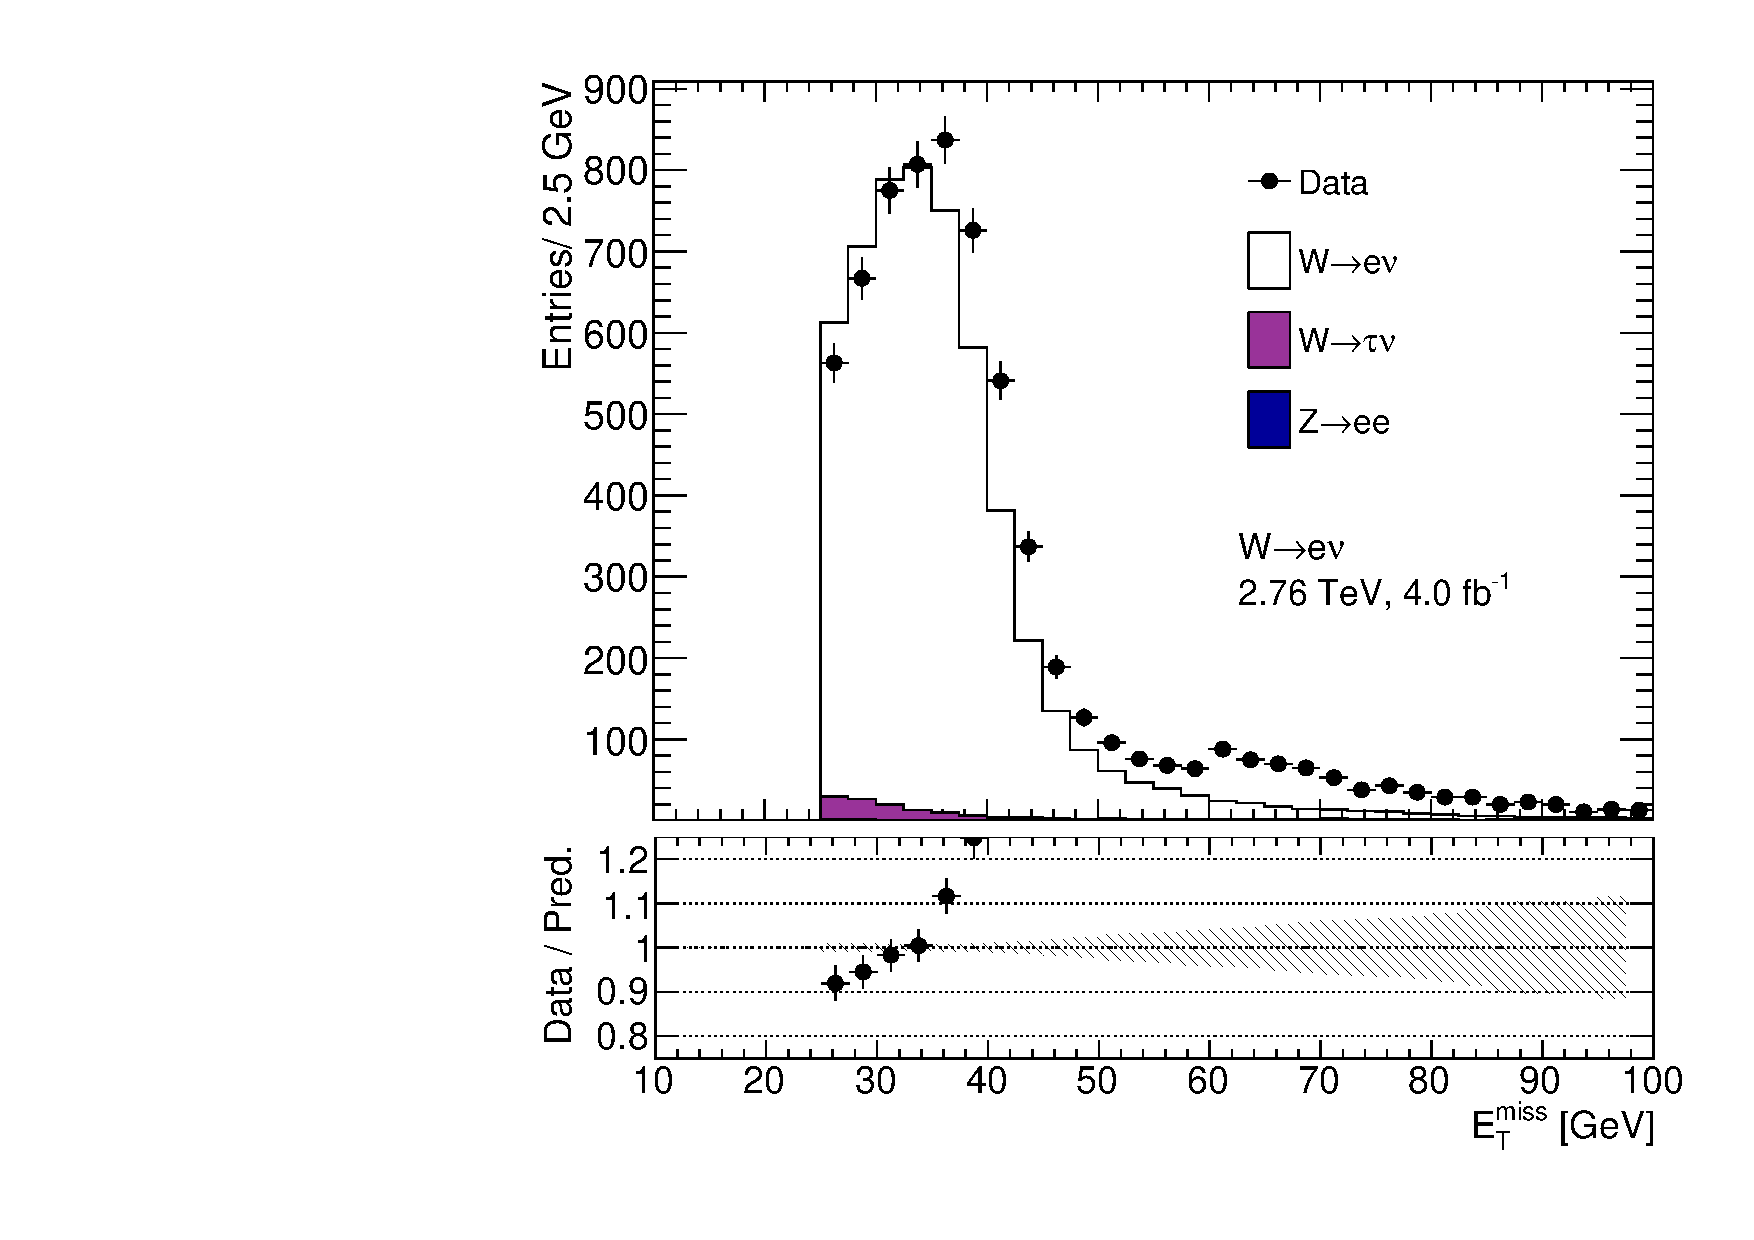
\includegraphics[width=1.\linewidth]{HadronRecoil/WenuRefFinal.pdf} \\ a)}
\end{minipage}
\hfill
\begin{minipage}[h]{0.49\linewidth}
\center{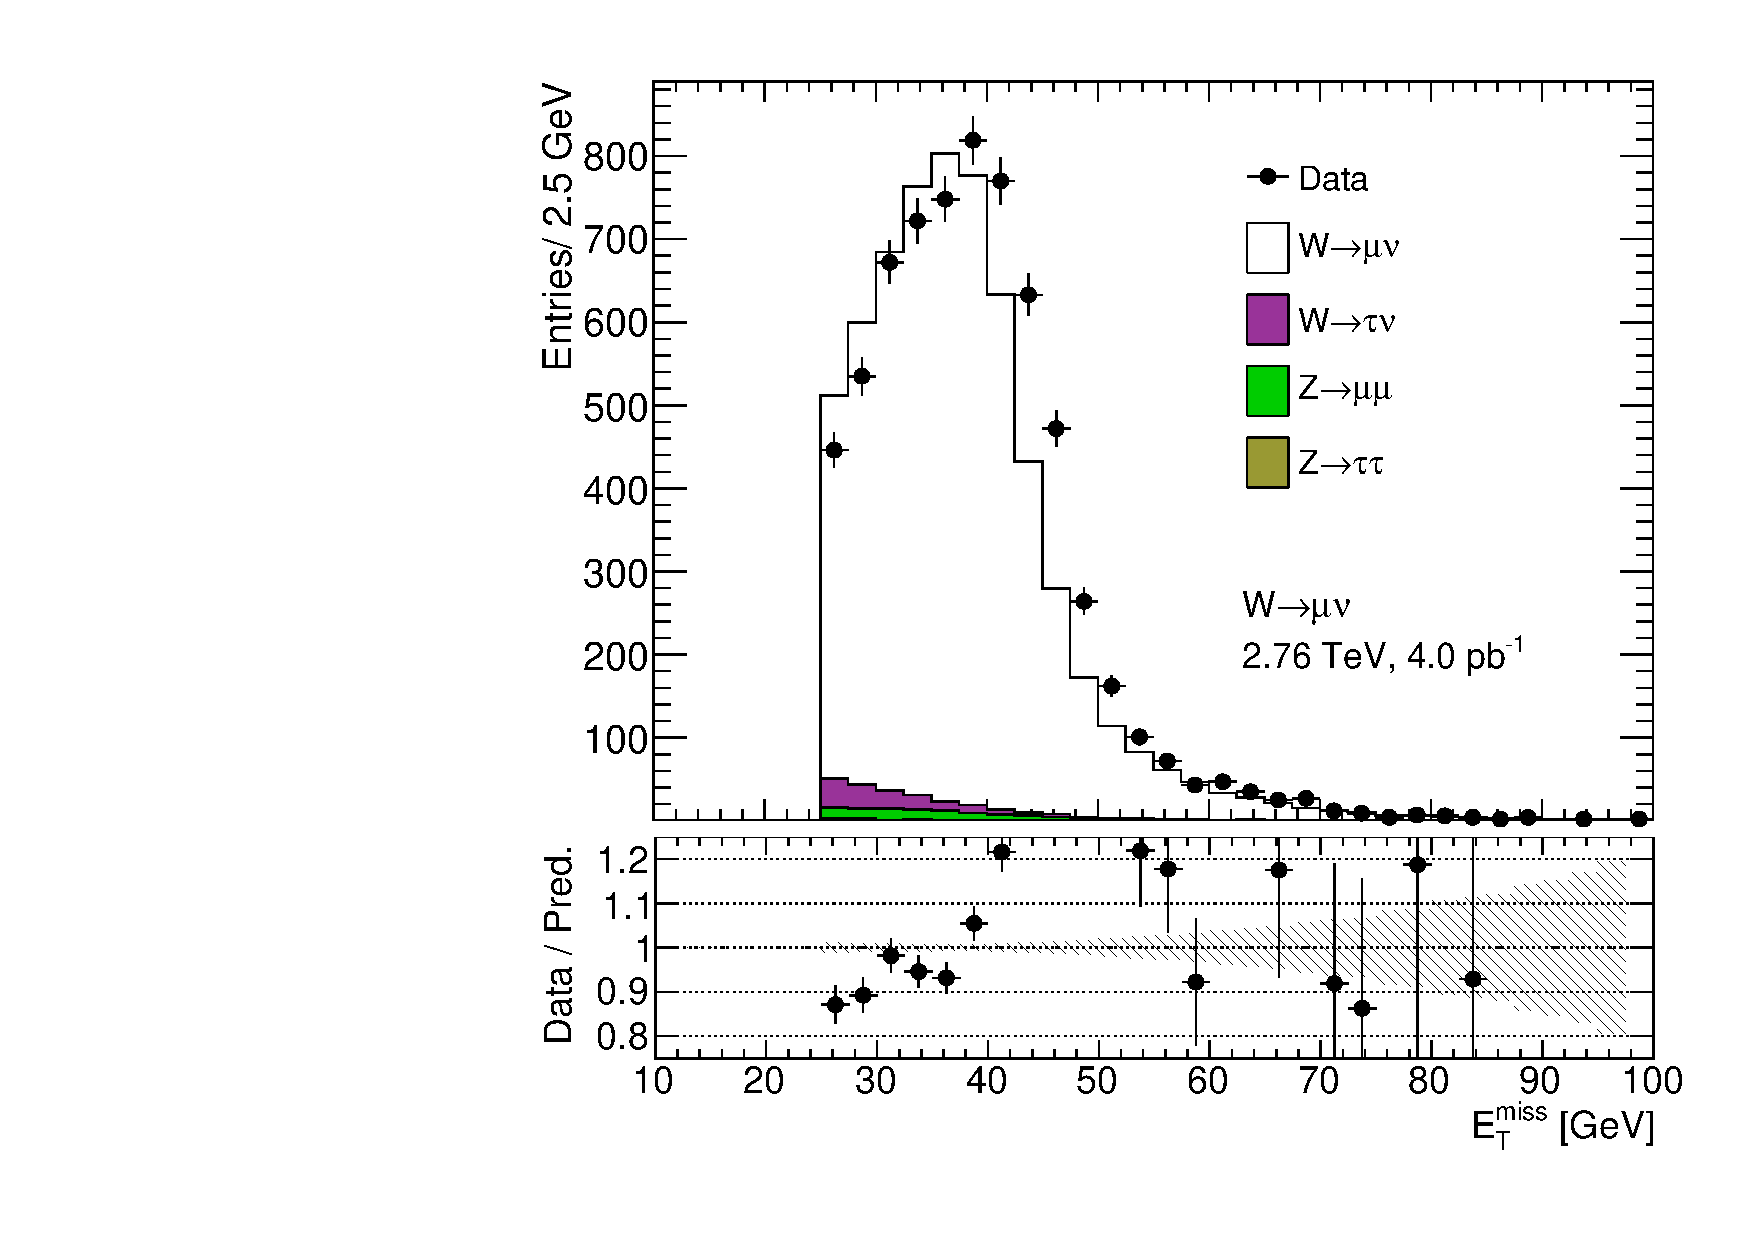
\includegraphics[width=1.\linewidth]{HadronRecoil/WmunuRefFinal.pdf} \\ b)}
\end{minipage}
\caption{Missing transverse energy distribution for a) the \wenu selection and  b) the \wmunu selection (described in Chap.~\ref{chap:EventSelection}). \etmiss is calculated using the standard \atlas algorithm. The expected contributions from all backgrounds are estimated with Monte Carlo simulations, except for multijet background that is not included. All Monte Carlo corrections from Chap.~\ref{chap:MCCor} are applied. There are visible discrepancies between data and MC, that cannot be explained by the contribution of the multijet background, which is expected to contribute mostly in the low \etmiss region (see Sec.~\ref{sec:QCD}).}
\label{ris:EtMissRefFinal}
\end{figure}

Standard reconstruction of \etmiss in the \atlas experiment \cite{Aad2012} uses transverse energy deposits in the calorimeter ($E_{x(y)}^{miss, calo}$), energy losses in cryostat ($E_{x(y)}^{miss, cryo}$)  and reconstructed muons ($E_{x(y)}^{miss, muon}$) for a calculation of:
\begin{equation}
E_{x(y)}^{miss} = E_{x(y)}^{miss, calo} +  E_{x(y)}^{miss, cryo} +  E_{x(y)}^{miss, muon}.
\end{equation}

The calorimeter-related $E_{x(y)}^{miss, calo}$ term uses the information about matched physics object for the cell calibration and can be defined as:
\begin{equation}
E_{x(y)}^{miss, calo} = E_{x(y)}^{miss, e} + E_{x(y)}^{miss, \gamma} + E_{x(y)}^{miss, \tau} + E_{x(y)}^{miss, jets} + E_{x(y)}^{miss,SoftTerm} + E_{x(y)}^{miss, \mu}.
\end{equation}
where each term is calculated from the negative sum of the calibrated cells energies inside the corresponding objects. Each jet with energy $P_T$>20 GeV is corrected for a pile-up and a jet energy scale is applied. Soft $E_{x(y)}^{miss,SoftTerm}$ term is calculated from clusters and tracks, that are not associated with physics objects. To avoid double counting, muon energy losses  in the calorimeter is  subtracted from \etmiss.  The muon $E_{x(y)}^{miss, \mu}$ term is calculated from the momenta of muons measured in a range of $| \eta | < 2.7 $. Since pile-up has a significant effect on \etmiss, several methods of pile-up suppression are used \cite{ATLAS-CONF-2014-019}.

The data used in the analysis is characterized by a low pile-up (Chap.~\ref{chap:DataSample}), so the usage of a standard \atlas procedure (optimized for high pile-up 8 TeV runs) is not optimal. It was observed, that there are big discrepancies between the \etmiss distributions for data and MC simulation, as shown in Fig.~\ref{ris:EtMissRefFinal}, where the missing transverse energy distribution for data is compared to signal and background MC predictions. 

The differences are visible in both the electron and muon channels and cannot be explained by the contribution from the missing multijet background, which is expected mainly in the low \etmiss region (see Sec.~\ref{sec:QCD} for more details). 



\subsection{Hadronic recoil}


An alternative method to calculate \etmiss  was developed in \cite{HadrRecoilFirst}. This procedure is based on a requirement of a balance in the transverse momentum of a W-boson and the initial (quark-gluon) state radiation:
\begin{equation}
\vec{P}_{T}^{W} = \vec{P}_T^l+\vec{P}_T^{\nu}= \sum{\vec{P}_{T}^{ISRquarks,gluon}}=HR, 
\end{equation}
where $\sum{\vec{P}_{T}^{ISRquarks,gluon}}$ is a transverse momentum of partons from the initial state radiation, also called hadronic recoil (HR) and $\vec{P}_T^l$, $\vec{P}_T^{\nu}$ are the transverse momenta of lepton and neutrino respectively. Therefore, \etmiss can be determined using the relation:
\begin{equation}
E_{T}^{miss} = - P_T^{\nu} =  - HR + \ptl.
\end{equation} 

This procedure assumes, that recoil arises from one single leading jet, and the rest  is coming from a soft hadronic activity. The hadronic recoil is computed as a vector sum of calorimeter clusters:
\begin{equation}
HR= \sum_{i=0}^{N_{topo}}\vec{P}_T^{topo},
\end{equation}
while a scalar sum of cluster energies in the transverse plane corresponds to the hadronic activity in the event:
\begin{equation}\label{eq:sumet}
\sum E_T =\sum_{i=0}^{N_{topo}} E_T^{topo}.
\end{equation}
To avoid double counting due to lepton energy lose in the calorimeter, the clusters energy inside a cone with a radius of $dR$ = 0.2 around the lepton direction are excluded from the calculation. To compensate subtracted soft activity from a cone, a replacement cone is added (Fig.~\ref{ris:subsCone}). This cone is defined as a cone at the same pseudorapidity but at a different $\phi$ and away from any other lepton and hadronic recoil direction. The cone is then rotated to the original lepton direction. 

\begin{figure}[!tbp]
\begin{center}
\begin{minipage}[h]{0.49\linewidth}
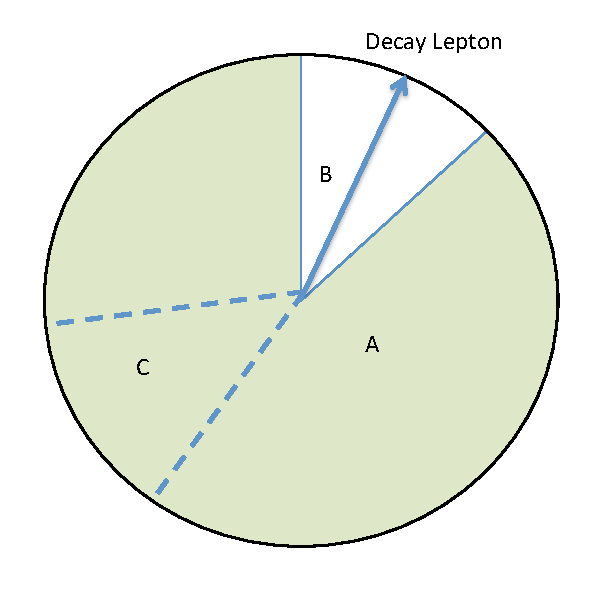
\includegraphics[width=1\textwidth]{HadronRecoil/ReplacementCluster.pdf}
\end{minipage}

\caption{Definition of different zones in the calculation of the cluster-based hadronic recoil. Zone B is excluded from hadronic recoil calculation because it contains decay lepton. To describe properly the overall activity it is replaced by the zone C, rotated in the direction of B. Zone A corresponds to the rest of the calorimeter\cite{HRPlots}.}
\label{ris:subsCone}
\end{center}
\end{figure}

Fig.~\ref{ris:HadrRecoilEtMiss} shows the control plots for the distributions of missing transverse energy calculated using the hadronic recoil procedure. In both the electron and muon channels the agreement between data and MC simulation is much better than in the case of the standard procedure (Fig.~\ref{ris:EtMissRefFinal}).  Therefore it is decided to use hadronic recoil \etmiss reconstruction method for the data sample used in the analysis.


\begin{figure}[!tbp]
\begin{minipage}[h]{0.49\linewidth}
\center{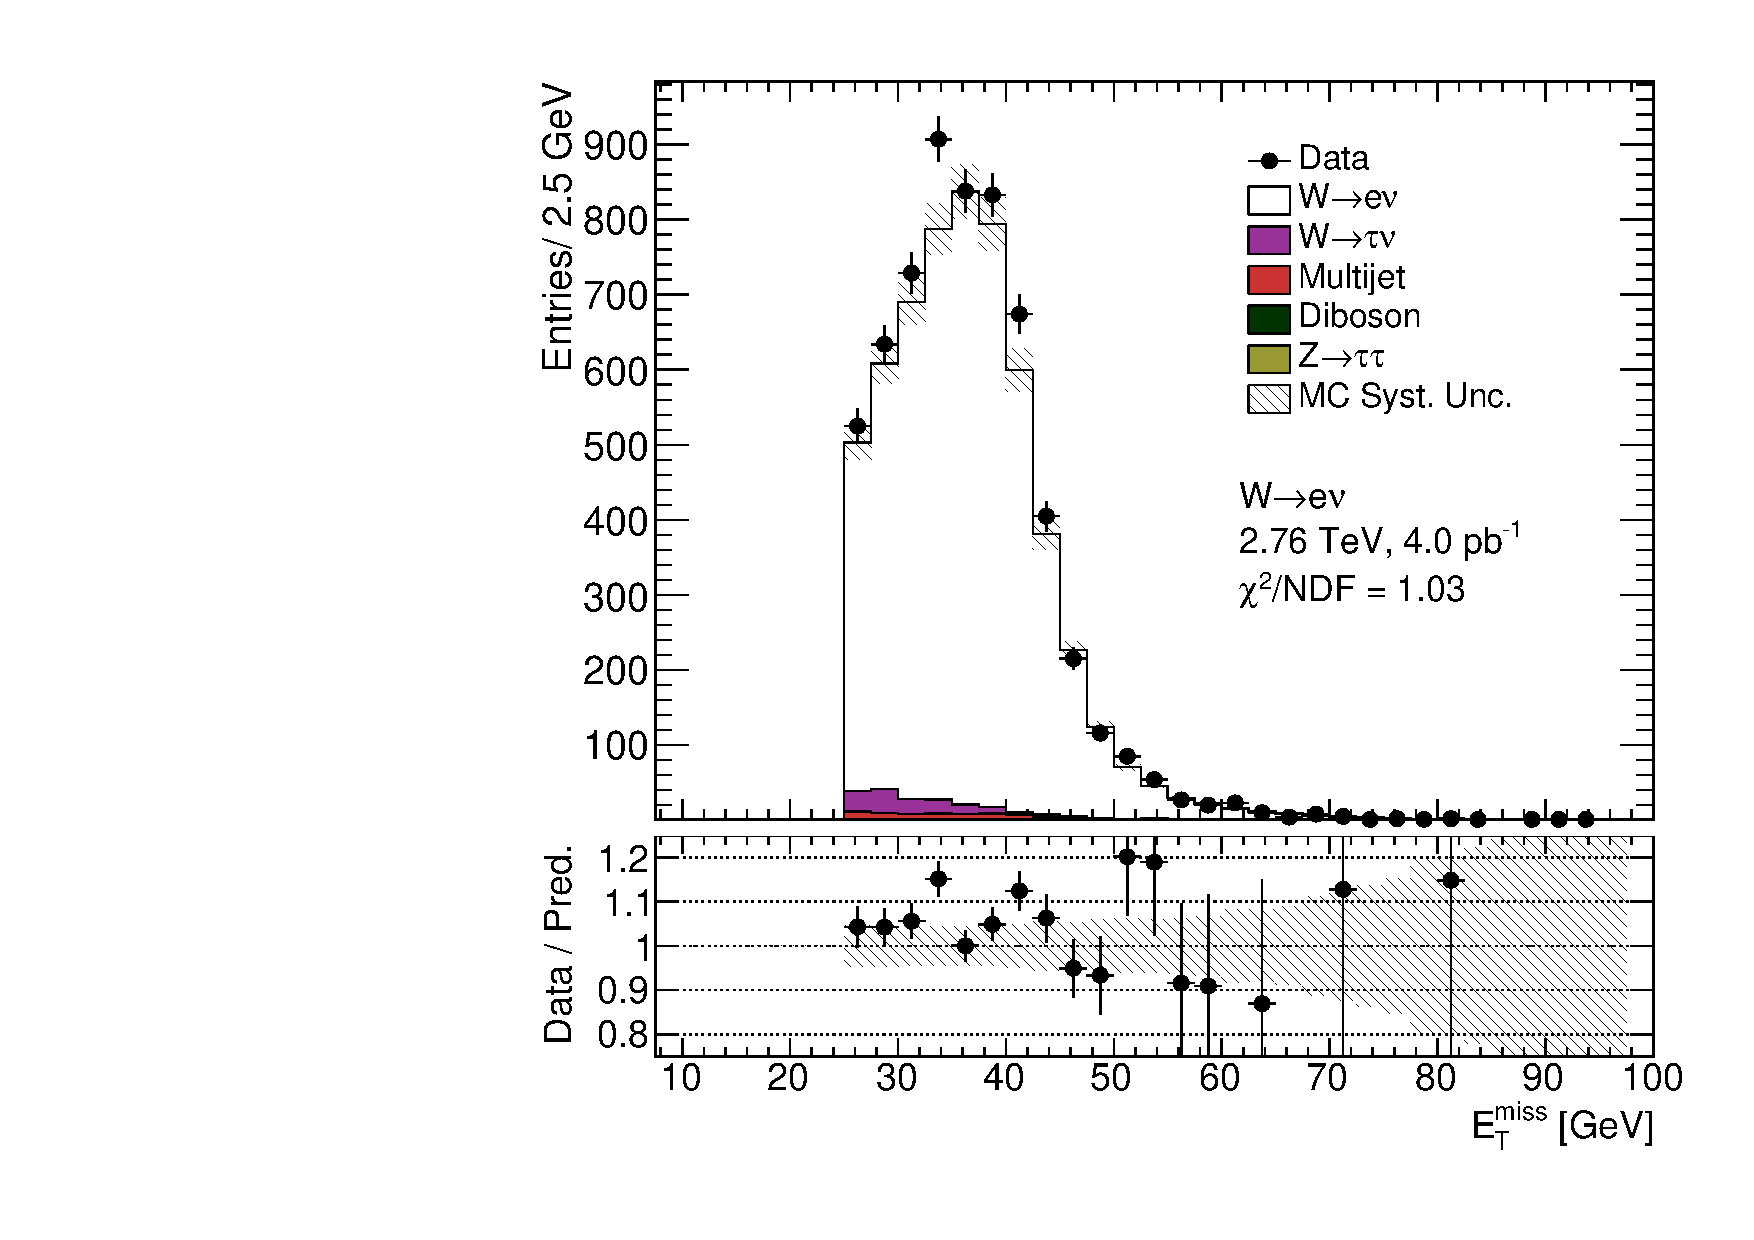
\includegraphics[width=1.\linewidth]{HadronRecoil/W_Boson_etMiss.pdf} \\ a)}
\end{minipage}
\hfill
\begin{minipage}[h]{0.49\linewidth}
\center{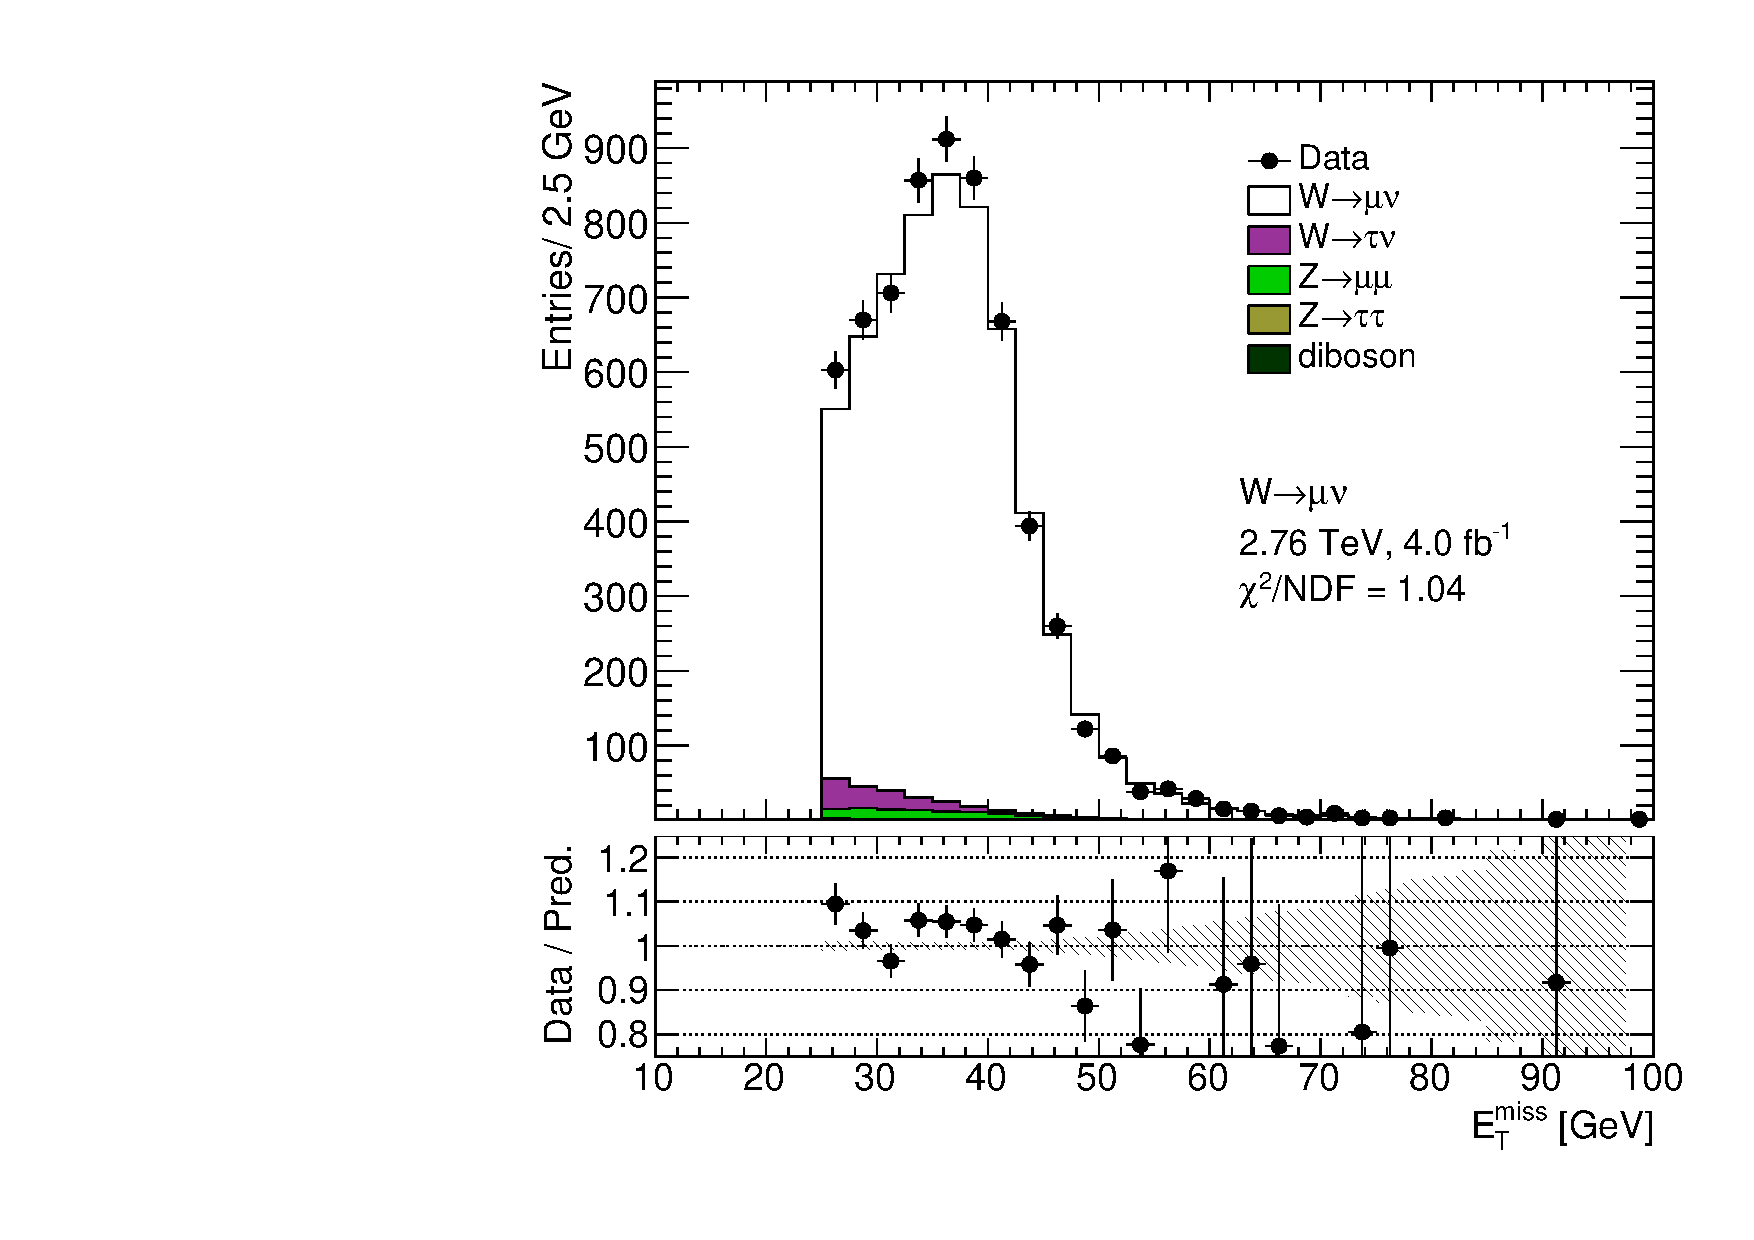
\includegraphics[width=1.\linewidth]{HadronRecoil/Wmu_Boson_etMiss.pdf} \\ b)}
\end{minipage}
\caption{Missing transverse energy distribution for a) the \wenu selection and  b) the \wmunu selection (described in Chap.~\ref{chap:EventSelection}). \etmiss  calculated using the hadronic recoil algorithm. The expected contributions from all backgrounds are estimated with Monte Carlo simulations, except for multijet background that is not included. All Monte Carlo corrections from Chap.~\ref{chap:MCCor} are applied.}
\label{ris:HadrRecoilEtMiss}
\end{figure}


